\section{Design concepts and selection}
\label{sec:concepts}

We considered only a handful of alternatives, and dropped each of them quickly. A hinged wedge, passive or spring-loaded, would have kept the wedge edge on the ramp surface, but fixed forks do the same job more simply and better (Section~\ref{sec:wedge}). A servo linkage bracing against both walls, and a side lifter to tip an opponent over the guide rail, were both too complex for the time we had, and an autonomous robot has no good way to know when to fire a lifter. Tennis grip tape on the tracks would have raised traction, but it slipped off because of the angle the tracks sit at (Section~\ref{sec:traction}).

What we built is a tracked robot with a forks-and-wedge front end that runs along a guide rail (Fig.~\ref{fig:robot}). The front end has no moving parts: on the mesa it turns an opponent's own drive force into the thing that removes it.

\begin{figure}[htbp]
  \centering
  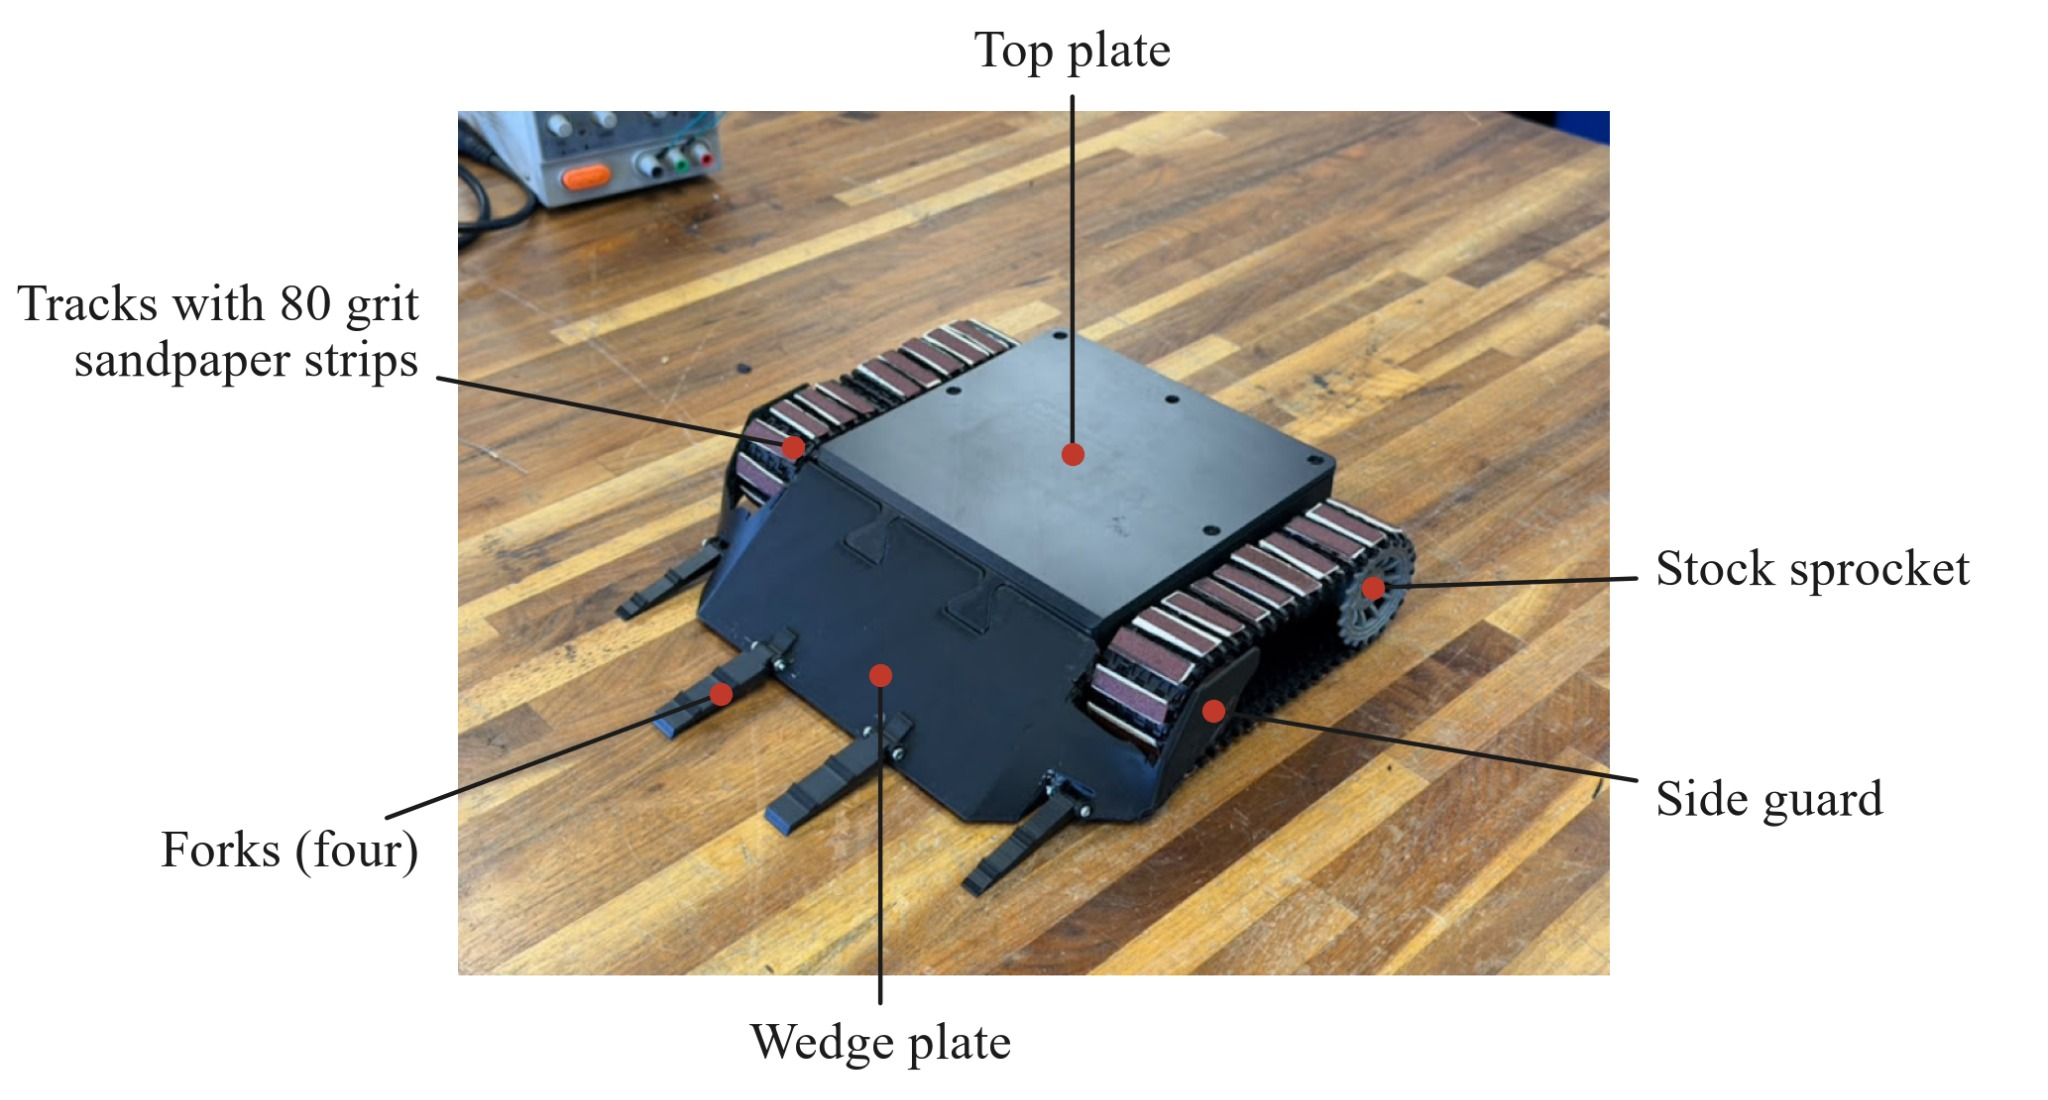
\includegraphics[width=\textwidth]{fig02_robot.jpg}
  \caption{The robot as built. A low wedge plate with four forks leads, the tracks carry strips of 80 grit sandpaper, and side guards run along each side.}
  \label{fig:robot}
\end{figure}
